
%(BEGIN_QUESTION)
% Copyright 2006, Tony R. Kuphaldt, released under the Creative Commons Attribution License (v 1.0)
% This means you may do almost anything with this work of mine, so long as you give me proper credit

Forklar virkemåten til denne reguleringskretsen, inkludert funksjonen til begge potensiometrene, og avgjør hvor disse potensiometrene bør settes for å oppnå ``strammest'' temperaturregulering (som gir størst mulig nærhet til settpunktstemperaturen over tid). Husk at et {\it termoelement} genererer en liten spenning proporsjonal med temperatur:

$$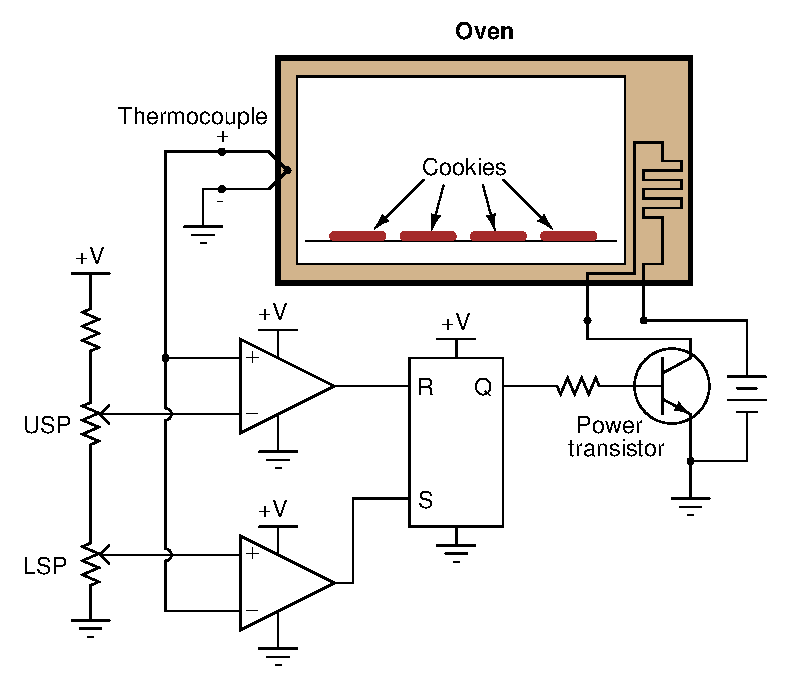
\includegraphics[width=15.5cm]{i01451x01.eps}$$

\underbar{file i01451}
%(END_QUESTION)





%(BEGIN_ANSWER)

To potensiometre gir doble settpunkter som spenningskomparatorene reagerer på. Dersom prosessverdisignalet (termoelementets utgangsspenning) er lavere enn nedre settpunkt, metter den nedre op-ampen ``høyt'', aktiverer ``Set''-inngangen på S-R-låsen og kobler inn effekt til varmeelementet.

Når ovnstemperaturen ligger mellom de to settpunktene (LSP $<$ PV $<$ USP), vil begge op-amp-utgangene være i ``lav'' tilstand, og S-R-låsen holder sin forrige utgangstilstand på Q.

Når prosessverdien overstiger øvre settpunkt, metter den øvre op-ampen ``høyt'', aktiverer ``Reset''-inngangen på S-R-låsen og kobler ut effekt til varmeelementet.

\vskip 10pt

Kort sagt er dette et enkelt {\it differensialgap}-reguleringssystem for en kjeksovn. For strammest mulig temperaturregulering settes LSP-potensiometeret til maksimum (helt {\it opp}) og USP-potensiometeret til minimum (helt {\it ned}).

%(END_ANSWER)





%(BEGIN_NOTES)

$$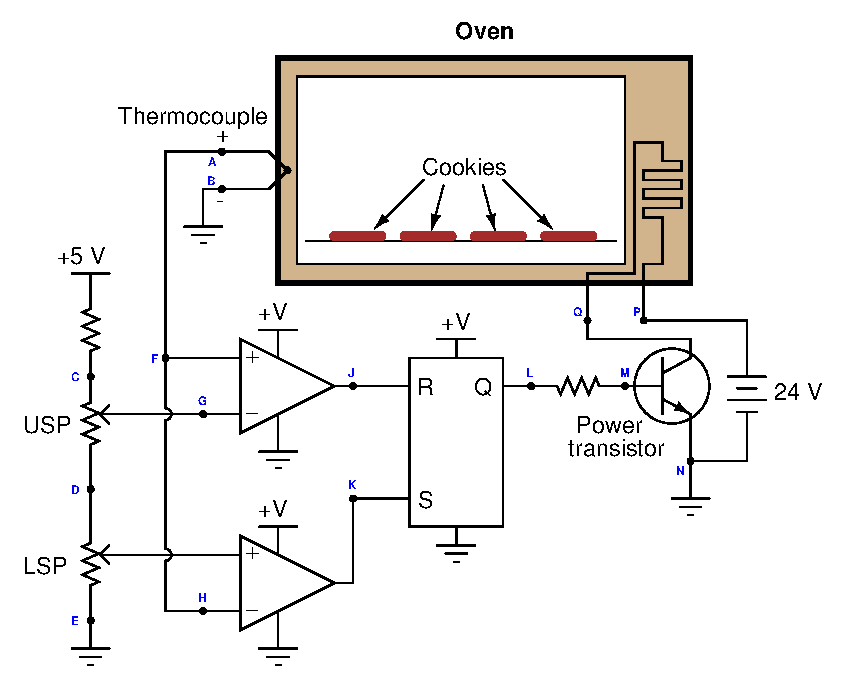
\includegraphics[width=15.5cm]{i01451x02.eps}$$

\vskip 20pt \vbox{\hrule \hbox{\strut \vrule{} {\bf Virtuell feilsøking} \vrule} \hrule}

Dette spørsmålet egner seg godt som en ``Virtuell feilsøking''-øvelse. Når du presenterer diagrammet for studentene, forestiller du deg først en bestemt feil i systemet. Deretter presenterer du ett eller flere symptomer på denne feilen (noe en operatør eller annen bruker kan observere). Studentene foreslår så ulike diagnostiske tester for å identifisere feilens natur og plassering, slik teknikere ville gjort i praktisk feilsøking. Din oppgave er å fortelle hva resultatet ville blitt for hver foreslått test, og dokumentere resultatene slik at alle studentene kan se dem.

Under og etter øvelsen er det nyttig å stille oppfølgingsspørsmål som:

\begin{itemize}
\item{} Hva forteller resultatet av den siste diagnostiske testen deg om feilen?
\item{} Anta at resultatene av den siste diagnostiske testen var annerledes. Hva ville det resultatet fortalt deg om feilen?
\item{} Er den siste diagnostiske testen den beste vi kunne gjort?
\item{} Hva ville vært ideell testrekkefølge for å diagnostisere problemet i færrest mulig trinn?
\end{itemize}

%INDEX% Control, basics: differential gap control (electronic)

%(END_NOTES)

